%%% LaTeX Template: Article/Thesis/etc. with colored headings and special fonts
%%%
%%% Source: http://www.howtotex.com/
%%% Feel free to distribute this template, but please keep to referal to http://www.howtotex.com/ here.
%%% February 2011
%%%
%%% Modified January 2016 by CDM
%%%  Preamble
\documentclass[11pt,letterpaper]{article}
\usepackage[margin=1.0in]{geometry}
\usepackage[T1]{fontenc}
\usepackage[bitstream-charter]{mathdesign}
\usepackage[latin1]{inputenc}					
\usepackage{amsmath}						
\usepackage{xcolor}
\usepackage{cite}
\usepackage{hyphenat}
\usepackage{graphicx}
\usepackage{float}
\usepackage{subfigure}
\usepackage{sectsty}
\usepackage[compact]{titlesec} 
\usepackage[tablegrid]{vhistory}
\usepackage{pbox}
\allsectionsfont{\color{accentcolor}\scshape\selectfont}
%%% Definitions
\definecolor{accentcolor}{rgb}{0.0,0.0,0.5} 
\newcommand{\teamname}{Team Hawt-Wheels}
\newcommand{\productname}{Smart Cart}
\newcommand{\coursename}{CSE 4317: Senior Design II}
\newcommand{\semester}{SUMMER 2016}
\newcommand{\docname}{Detailed Design Specification}
\newcommand{\department}{Department of Computer Science \& Engineering}
\newcommand{\university}{The University of Texas at Arlington}
\newcommand{\authors}{Brian Wong \\ David Harvey \\ Dennis Otieno \\ Peggy Soh \\ Or Zoarets}

%%% Headers and footers
\usepackage{fancyhdr}
	\pagestyle{fancy}						% Enabling the custom headers/footers
\usepackage{lastpage}	
	% Header (empty)
	\lhead{}
	\chead{}
	\rhead{}
	% Footer
	\lfoot{\footnotesize \teamname \ - \semester}
	\cfoot{}
	\rfoot{\footnotesize page \thepage\ of \pageref{LastPage}}	% "Page 1 of 2"
	\renewcommand{\headrulewidth}{0.0pt}
	\renewcommand{\footrulewidth}{0.4pt}

%%% Change the abstract environment
\usepackage[runin]{abstract}			% runin option for a run-in title
%\setlength\absleftindent{30pt}			% left margin
%\setlength\absrightindent{30pt}		% right margin
\abslabeldelim{\quad}	
\setlength{\abstitleskip}{-10pt}
\renewcommand{\abstractname}{}
\renewcommand{\abstracttextfont}{\color{accentcolor} \small \slshape}	% slanted text

%%% Start of the document
\begin{document}

%%% Cover sheet
{\centering \huge \color{accentcolor} \sc \textbf{\department \\ \university} \par}
\vspace{1 in}
{\centering \huge \color{accentcolor} \sc \textbf{\docname \\ \coursename \\ \semester} \par}
\vspace{0.5 in}
\begin{figure}[h!]
	\centering
   	
\includegraphics[width=0.60\textwidth]{images/smart_cart_logo}
\end{figure}
\vspace{0.5 in}
{\centering \huge \color{accentcolor} \sc \textbf{\teamname \\ \productname} \par}
\vspace{0.5 in}
{\centering \large \sc \textbf{\authors} \par}
\newpage


%\vspace{1 in}
%\centerline{January 13th, 2012}
%\newpage

%%% Revision History
\begin{versionhistory}
  	\vhEntry{0.1}{08.01.2016}{DO|OZ}{Document Creation}
  	\vhEntry{0.2}{08.17.2016}{PS|BW}{Complete Draft}
\end{versionhistory}
\newpage

%%% Table of contents
\setcounter{tocdepth}{2}
\tableofcontents
\newpage

%%% List of figures and tables (optional)
\listoffigures
\listoftables
\newpage

%%% Document sections
\section{Introduction}
\subsection{Product Concept}
The Smart Cart will provide assistance by being an autonomous carrier. The cart needs to be able to do the following things:
\begin{itemize}
	\item Follow a ''master'' to the designated destination
	\item Avoid collision with obstacles such as walls and other people
	\item Include an integrated power supply
	\item Holonomic mobility
\end{itemize}

\subsection{Scope}
The main function of the Smart Cart is to help its user carry tools from one point to another. It will also have an integrated power supply to allow its user to charge or power his or her tools. A unique feature of the Smart Cart is that the cart will identify and follow its "master" by using the Intel RealSense. Another unique feature of the cart is its holonomic wheels. This allows the cart to easily maneuver and avoid collisions with objects by using image processing from a camera. The Smart Cart will require external input from the user. The user must wear a colored band that is provided with the Smart Cart. This band is used by the cart for tracking its "master". External outputs produced by the cart will be messages to let its user know whether it has succesfully identified its master. There are no other external inputs or outputs. A simple user interface may be implemented for identification of master depending on the availability of time. 

\subsection{Key Requirements}
The Smart Cart shall have five layers that work in unison to allow the cart to autonomously navigate and follow a specified user. The five layers in the system are the Smart Cart layer, Power Supply layer, Imaging/Navigation layer and Crab Drive layer. The five layers will be discussed more in the following sections.
\section{System Overview}
This section should describe the overall structure of your software system. Think of it as the strategy for how you will build the system. An architectural "layer" is the top-level logical view, or an abstraction, of your design. Layers should be composed of related elements of similar capabilities, and should be highly independent of other layers, but should have very clearly defined interfaces and interactions with other layers. Each layer should be identified individually and should be unique as to its function and purpose within the system. This section should also contain the high-level block diagram of the layers, as shown in the example below, as well as detailed descriptions of the functions of each layer.

\begin{figure}[h!]
	\centering
 	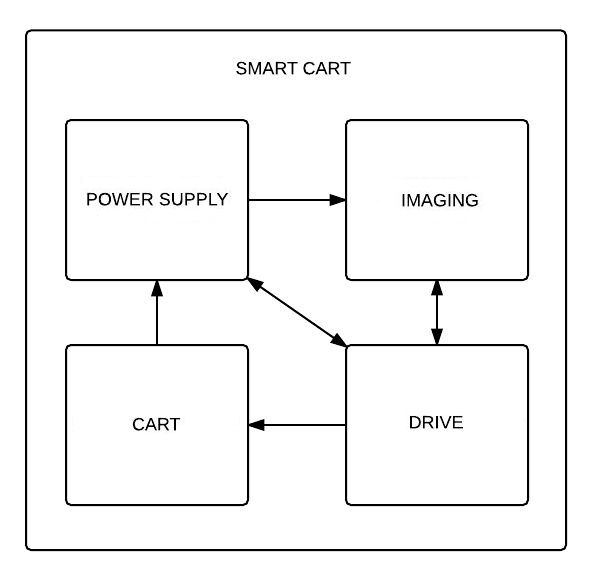
\includegraphics[width=0.60\textwidth]{images/system_overview}
 \caption{A simple architectural layer diagram}
\end{figure}


\subsection{Power Supply Layer Description}
Each layer should be described separately in detail. Descriptions should include the features, functions, critical interfaces and interactions of the layer. The description should clearly define the services that the layer provides. Also include any conventions that your team will use in describing the structure: naming conventions for layers, subsystems, modules, and data flows; interface specifications; how layers and subsystems are defined; etc.

\subsection{Cart Layer Description}
Each layer should be described separately in detail. Descriptions should include the features, functions, critical interfaces and interactions of the layer. The description should clearly define the services that the layer provides. Also include any conventions that your team will use in describing the structure: naming conventions for layers, subsystems, modules, and data flows; interface specifications; how layers and subsystems are defined; etc.

\subsection{Crab Drive Layer Description}
Each layer should be described separately in detail. Descriptions should include the features, functions, critical interfaces and interactions of the layer. The description should clearly define the services that the layer provides. Also include any conventions that your team will use in describing the structure: naming conventions for layers, subsystems, modules, and data flows; interface specifications; how layers and subsystems are defined; etc. 

\subsection{Imaging and Navigation Description}
Each layer should be described separately in detail. Descriptions should include the features, functions, critical interfaces and interactions of the layer. The description should clearly define the services that the layer provides. Also include any conventions that your team will use in describing the structure: naming conventions for layers, subsystems, modules, and data flows; interface specifications; how layers and subsystems are defined; etc. 
\newpage
%\section{Subsystem Definitions \& Data Flow}
%This section breaks down the simple architectural layer diagram with another level of detail. The logical subsystems that compose each layer and its interactions and interfaces between the subsystems are graphically represented. Even though the power supply layer does not have data flow, it is still a key layer to the system. The following data flow block diagram shows a high level diagram of all the layers in the Smart Cart.

\begin{figure}[h!]
	\centering
 	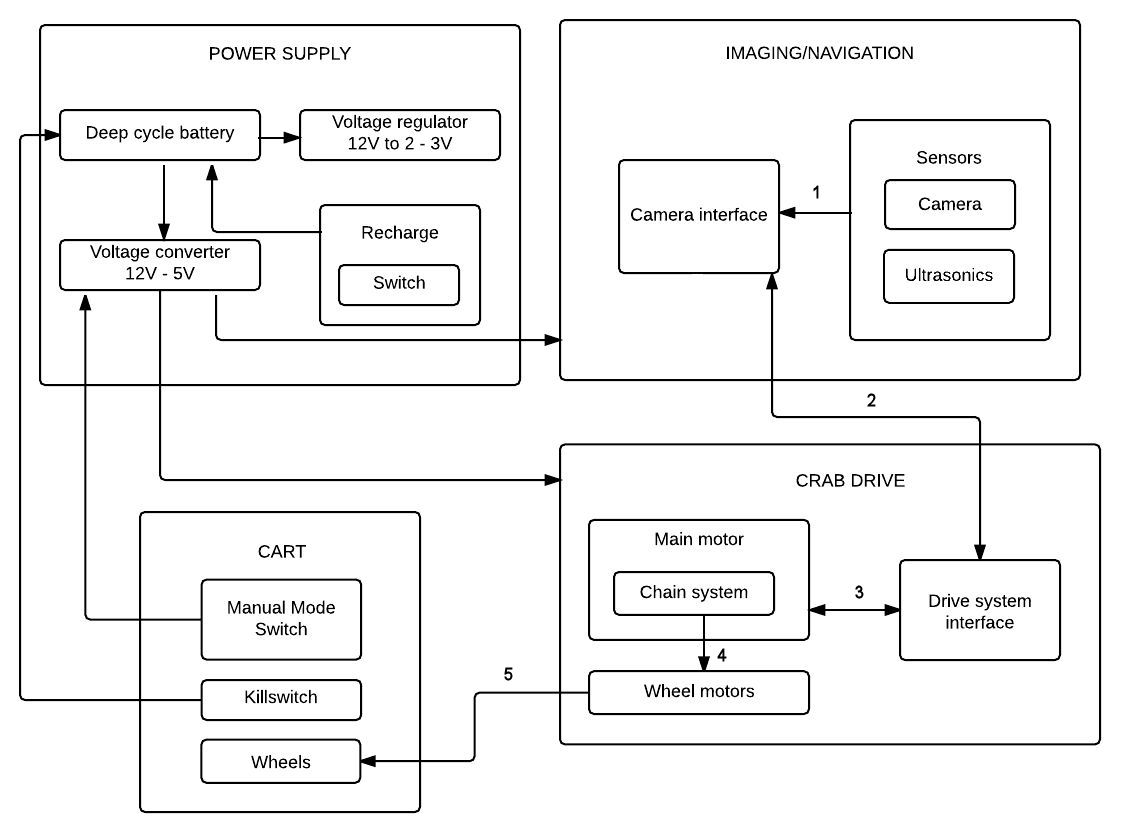
\includegraphics[width=\textwidth]{images/diagram_whole}
 \caption{A simple data flow diagram}
\end{figure}

\newpage
\section{POWER SUPPLY SUBSYSTEM}
The power supply layer is one of the most important layers because it provides stable power supply
to the cart. The parts in this subsystem are responsible for powering every other subsystem and any
external tools or equipment.

\subsection{DEEP CYCLE BATTERY}
A rechargeable battery that will provide consistent power up to 12 V.
\begin{figure}[h!]
	\centering
 	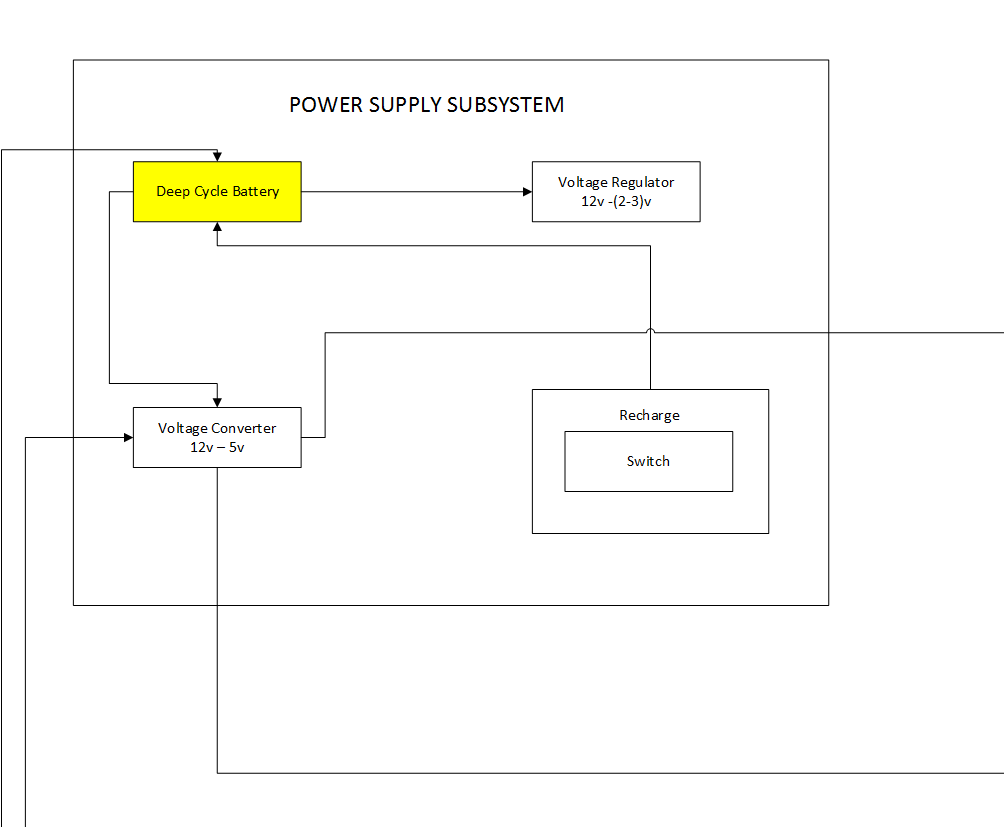
\includegraphics[width=0.60\textwidth]{images/battery}
 \caption{Deep Cycle Battery Subsystem description diagram}
\end{figure}

\subsubsection{ASSUMPTIONS}
\begin{itemize}
\item The battery is charged.
\item The battery is properly connected to the cart
\item The battery is fully functional
\item The battery is connected to the cart at all times
\end{itemize}

\subsubsection{RESPONSIBILITIES}
The deep cycle battery subsystem responsibilities are as follows:
\begin{itemize}
\item Provide stable power supply to the other subsystems after being converted from 12v to 5v by the voltage converter.
\item Enable stable power to external tools and equipment after being converted from 12V to 2 - 3V through the voltage regulator.
\end{itemize}

\subsubsection{SUBSYSTEM INTERFACES}
\begin {table}[H]
\caption {Deep cycle battery subsystem interfaces} 
\begin{center}
    \begin{tabular}{ | p{1cm} | p{6cm} | p{3cm} | p{3cm} |}
    \hline
    ID & Description & Inputs & Outputs \\ \hline
    \ N/A & Power integrated power supply & \pbox{3cm}{N/A} & \pbox{3cm}{Voltage regulator }  \\ \hline
    \ N/A & Power electronic components & \pbox{3cm}{N/A} & \pbox{3cm}{Voltage converter}  \\ \hline
    \ N/A & Safety killswitch & \pbox{3cm}{Killswitch} & \pbox{3cm}{N/A}  \\ \hline
    \ N/A & Safety manual mode & \pbox{3cm}{Manual-mode switch} & \pbox{3cm}{N/A}  \\ \hline
    \end{tabular}
\end{center}
\end{table}

\subsection{VOLTAGE REGULATOR}
The voltage regulator is designed to convert the 12V voltage from the deep cycle battery to 2 - 3V and it will mainly be used to power up external tools and equipment.
\begin{figure}[h!]
	\centering
 	\includegraphics[width=0.60\textwidth]{images/voltageRegulator}
 \caption{Voltage Regulator Subsystem description diagram}
\end{figure}

\subsubsection{ASSUMPTIONS}
Assumptions made are as follows:
\begin{itemize}
\item The voltage from the battery will be 12v.
\item The voltage required fro external tools and equipment will be between 2-3v.
\end{itemize}

\subsubsection{RESPONSIBILITIES}
\begin{itemize}
\item To enable and regulate constant voltage level for powering external tools and supplies.
\end{itemize}

\subsubsection{SUBSYSTEM INTERFACES}
\begin {table}[H]
\caption {Voltage Regulator Subsystem Interfaces} 
\begin{center}
    \begin{tabular}{ | p{1cm} | p{6cm} | p{3cm} | p{3cm} |}
    \hline
    ID & Description & Inputs & Outputs \\ \hline
    \ N/A & Receive power & \pbox{3cm}{Deep Cycle Battery} & \pbox{3cm}{N/A }  \\ \hline
    \end{tabular}
\end{center}
\end{table}


\subsection{RECHARGE}
The Recharge subsystem will be used to to ensure that Smart Cart will be charged without having too much electricity going to the battery or other cart components
\begin{figure}[h!]
	\centering
 	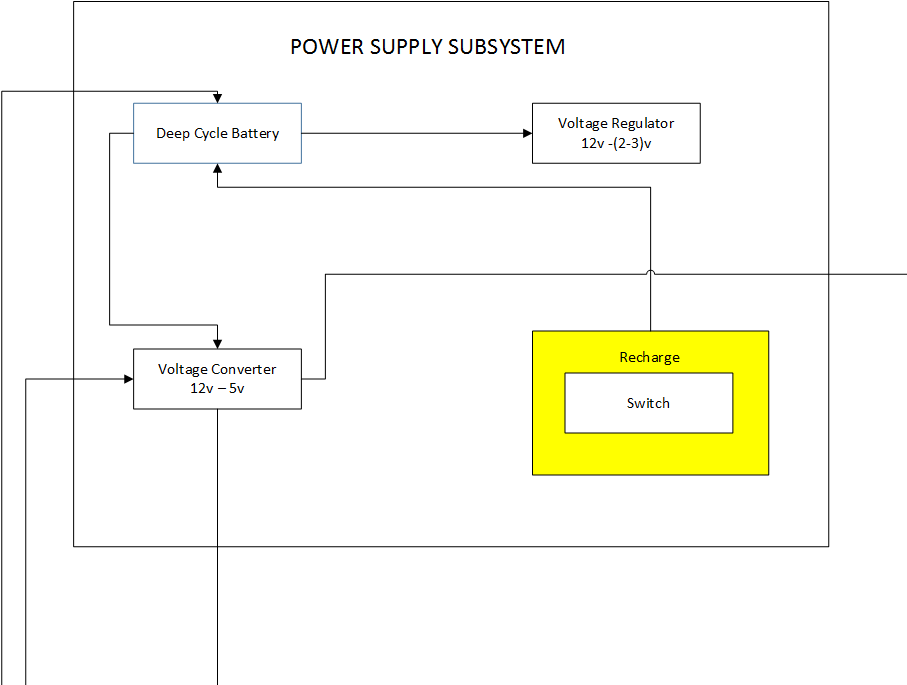
\includegraphics[width=0.60\textwidth]{images/recharge}
 \caption{Recharge Subsystem}
\end{figure}

\subsubsection{ASSUMPTIONS}
Assumptions are as follows:

\begin{itemize}
\item The Recharge subsystem will ensure the safety of the tools and equipment.
\end{itemize}

\subsubsection{RESPONSIBILITIES}
The responsibilities of the Recharge subsystem are as follows:

\begin{itemize}
\item A switch will disable the battery from the powering the Smart Cart components while it is being charged
\end{itemize}

\subsubsection{SUBSYSTEM INTERFACES}
\begin {table}[H]
\caption {Recharge Subsystem Interfaces} 
\begin{center}
    \begin{tabular}{ | p{1cm} | p{6cm} | p{3cm} | p{3cm} |}
    \hline
    ID & Description & Inputs & Outputs \\ \hline
    \ N/A & Switch o safety & \pbox{3cm}{Switch} & \pbox{3cm}{Deep cycle battery}  \\ \hline
    \end{tabular}
\end{center}
\end{table}

\subsection{VOLTAGE CONVERTER}
The voltage regulatlor is designed to convert the 12V from the deep cycle battery to a 2-3V to be used to power up smart cart equipment
\begin{figure}[h!]
	\centering
 	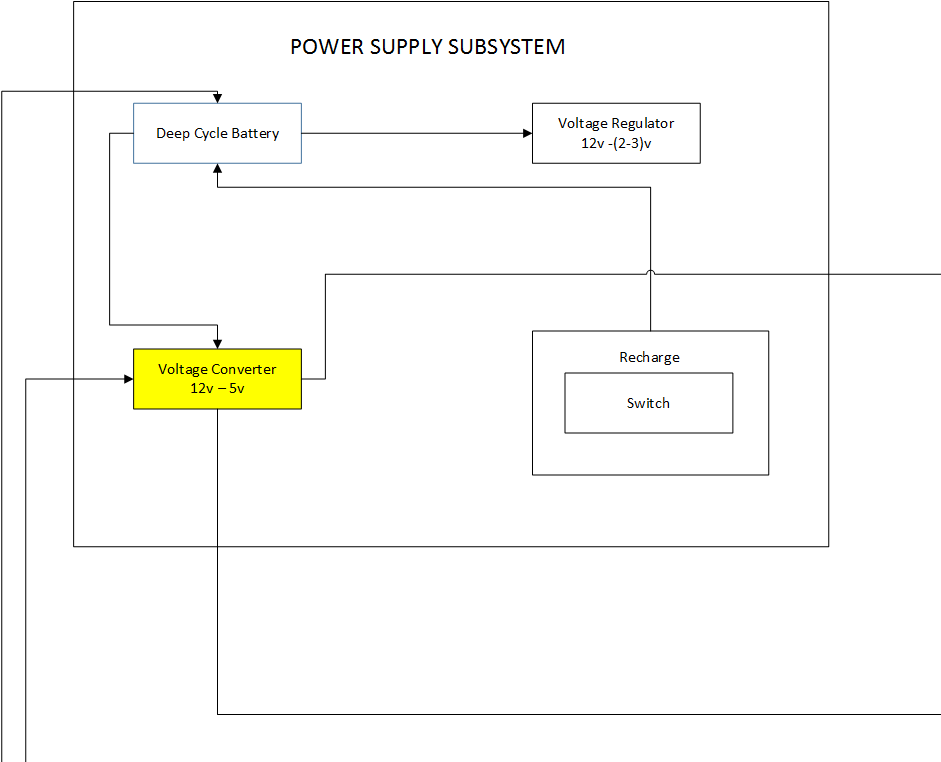
\includegraphics[width=0.60\textwidth]{images/voltageconverter}
 \caption{Voltage Converter Subsystem}
\end{figure}

\subsubsection{ASSUMPTIONS}
Assumptions made are as follows:
\begin{itemize}
\item The voltage from the battery will be 12V.
\item The voltage required by the cart's components will be 5V
\end{itemize}

\subsubsection{RESPONSIBILITIES}
The voltage converter subsystem responsibilities are as follows:
\begin{itemize}
\item Enable stable power to the other subsystems, which include the crab drive system and image processing after being converted from 12V to 5V through the voltage converter.
\end{itemize}

\subsubsection{SUBSYSTEM INTERFACES}

\begin {table}[H]
\caption {Voltage Converter Subsystem Interfaces} 
\begin{center}
    \begin{tabular}{ | p{1cm} | p{6cm} | p{3cm} | p{3cm} |}
    \hline
    ID & Description & Inputs & Outputs \\ \hline
    \ N/A & Receive Power &\pbox{3cm}{Deep Cycle battery} & \pbox{3cm}{N/A} \\ \hline
    \ N/A & Safety Manual Mode & \pbox{3cm}{Manual-mode switch} & \pbox{3cm}{Crab-drive system Imaging and Navigation }  \\ \hline
    \end{tabular}
\end{center}
\end{table}

\newpage
\section{IMAGING AND NAVIGATION SUBSYSTEM}
The imaging and navigation layer consists of the Intel RealSense Camera, ultrasonic sensors and imaging software to produce navigation data to be sent to the drive system interface. The navigation data that will direct the crab drive system to follow a user as well as obstacle avoidance

\subsection{SENSORS SUBSYSTEM}
Sensors include the Intel RealSense camera and ultrasonic sensors. The RealSense will identify a user to follow and the ultrasonic sensors will be used for obstacle avoidance. The sensors will provide the necessary information to the camera interface needed to create navigation data.

\begin{figure}[h!]
	\centering
 	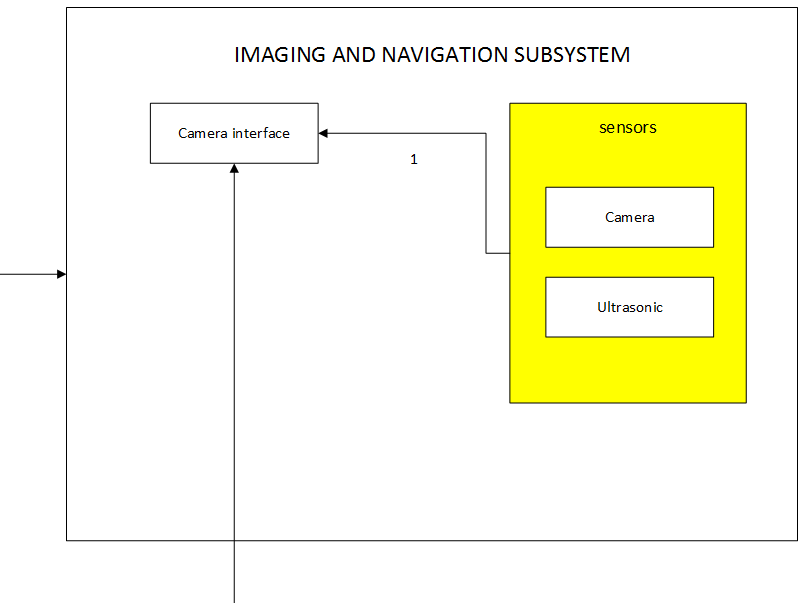
\includegraphics[width=0.60\textwidth]{images/sensors}
 \caption{Sensors subsystem description diagram}
\end{figure}

\subsection{ASSUMPTIONS}
Assumptions made are as follows:
\begin{itemize}
\item The user will be wearing a colored wristband that identifies them as the master
\item The user will stay in front of the Intel RealSense to avoid possible errors, such as the cart loosing vision of its master
\end{itemize}

\subsection{RESPONSIBILITIES}
The sensor subsystem responsibilities are as follows:
\begin{itemize}
\item Process image and ultrasonic data in real time
\item keep the designated master within the image frame
\item Gather accurate data to send to the camera interface
\end{itemize}
\subsection{SUBSYSTEM INTERFACES}
\begin{table}[H]
\caption{Sensors subsystem interface}
\begin{center}
\begin{tabular}{ | p{1cm} | p{6cm} | p{3cm} | p{3cm} |}
    \hline
    ID & Description & Inputs & Outputs \\ \hline
    \ 1 & Send sensor data & \pbox{3cm}{Camera Ultrasonic} & \pbox{3cm}{Camera interface }  \\ \hline
\end{tabular}
\end{center}
\end{table}

\subsection{CAMERA INTERFACE SUBSYSTEM}
The camera interface is responsible for receiving data from sensors and calculating the required navigation data and sending it to the crab drive's system interface. The navigation data will include require speed, direction needed and distance from obstacles.
\begin{figure}[h!]
	\centering
 	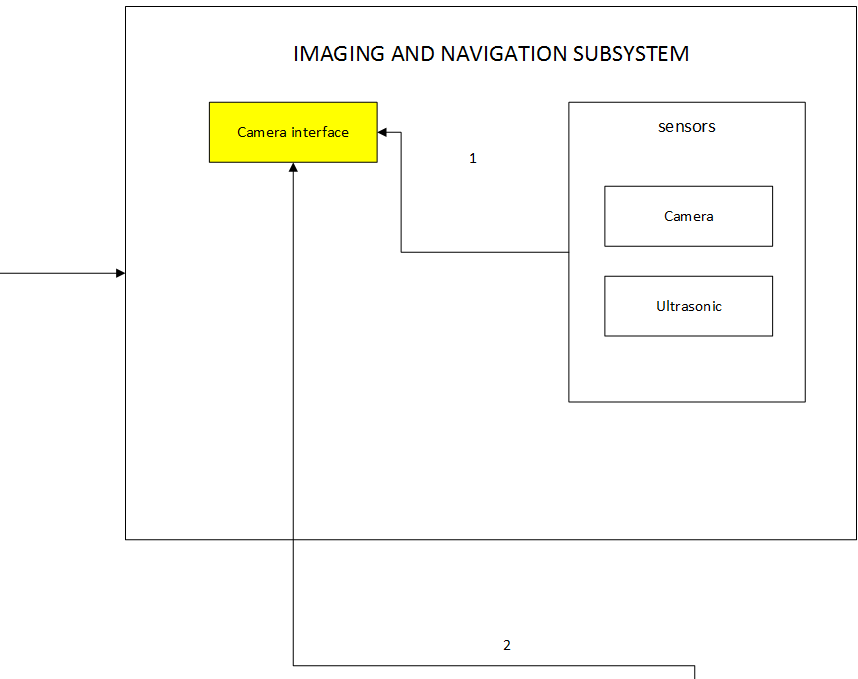
\includegraphics[width=0.60\textwidth]{images/camerainterface}
 \caption{Camera Interface subsystem description diagram}
\end{figure}

\subsection{ASSUMPTIONS}
Assumptions are as follows:
\begin{itemize}
\item Accurate data is being sent from the sensors
\item The camera interface will be able to communicate with the drive system interface 
\end{itemize}

\subsection{RESPONSIBILITIES}
The camera subsystem responsibility are as below:
\begin{itemize}
\item Calculate and process the navigation data
\item Communicate necessary information to the drive system interface 
\end{itemize}

\subsection{SUBSYSTEM INTERFACES}
\begin{table}[H]
\caption{Camera Interface Subsystem interfaces}
\begin{center}
\begin{tabular}{ | p{1cm} | p{6cm} | p{3cm} | p{3cm} |}
    \hline
    ID & Description & Inputs & Outputs \\ \hline
    \ 2 & Calculating navigation data & \pbox{3cm}{Sensors} & \pbox{3cm}{Drive System interface }  \\ \hline
\end{tabular}
\end{center}
\end{table}


\newpage
\section{CRAB DRIVE SUBSYSTEM}
The crab drive layer is a vital layer to this project. It's major function shall be to make Smart Cart mobile. It comprises comprises such vital elements as the micro-controller, the motor-controllers and the drive system interface.
\subsection{MOTOR CONTROL SUBSYSTEM}
The motor control subsystem will contain a roller chain that will be responsible for steering the the cart and maintain a consistent orientation for all the wheels, a central motor to coordinate the movement of the four wheels and wheel motors to drive the wheels
\begin{figure}[h!]
	\centering
 	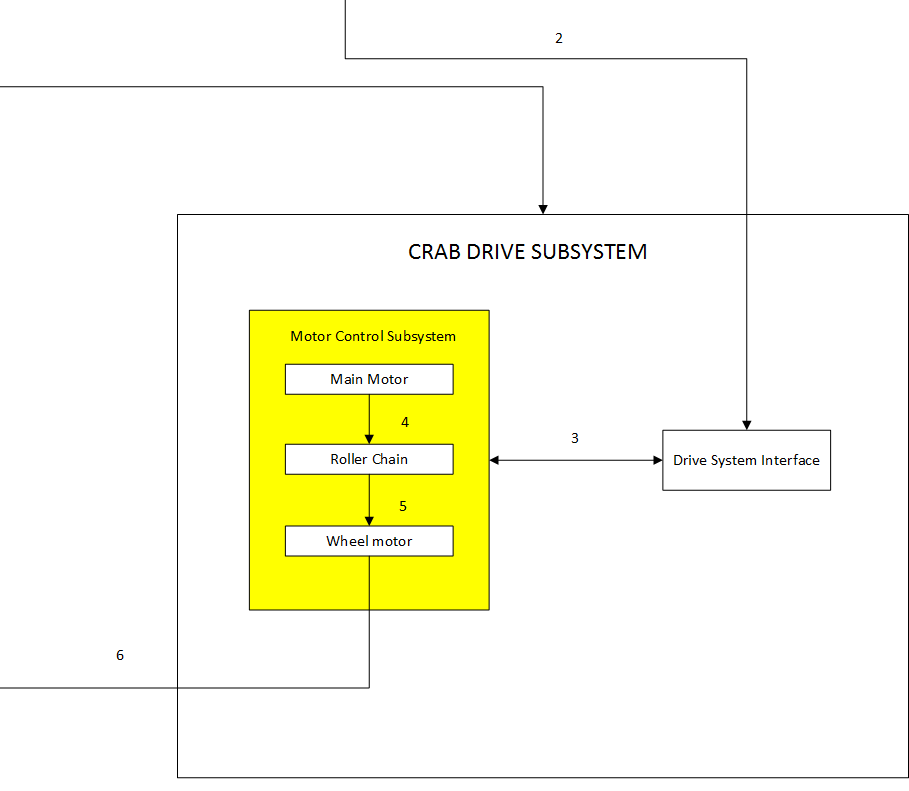
\includegraphics[width=0.60\textwidth]{images/motorcontrol}
 \caption{Motor Control subsystem description diagram}
\end{figure}

\subsection{ASSUMPTIONS}
Assumptions made are as follows:
\begin{itemize}
\item The main motor will correctly steer the wheels with the roller chain
\item The main motor will have a method to accurately keep wheel orientation data
\item The wheel motors will move the wheels accordingly
\end{itemize}

\subsection{RESPONSIBILITIES}
The main motor subsystem's responsibilities are as follows:
\begin{itemize}
\item Receive steering instructions from the drive system interface and accurately perform instructions.
\end{itemize}

\subsection{SUBSYSTEM INTERFACES}
\begin{table}[H]
\caption{Motor Control subsystem interface}
\begin{center}
\begin{tabular}{ | p{1cm} | p{6cm} | p{4cm} | p{4cm} |}
    \hline
    ID & Description & Inputs & Outputs \\ \hline
    \ 3 & Feedback data & \pbox{3cm}{N/A} & \pbox{4cm}{Drive system interface}  \\ \hline
    \ 6 & Steer Wheels & \pbox{3cm}{Drive system interface} & \pbox{4cm}{Wheel motors}  \\ \hline
\end{tabular}
\end{center}
\end{table}


\subsection{DRIVE SYSTEM INTERFACE SUBSYSTEM}
The drive system interface s designed to communicate with the navigation subsystem's camera interface it will get navigation data from the camera interface to steer the main drive motor as well as receiving feedback information for the wheel orientations.

\begin{figure}[h!]
	\centering
 	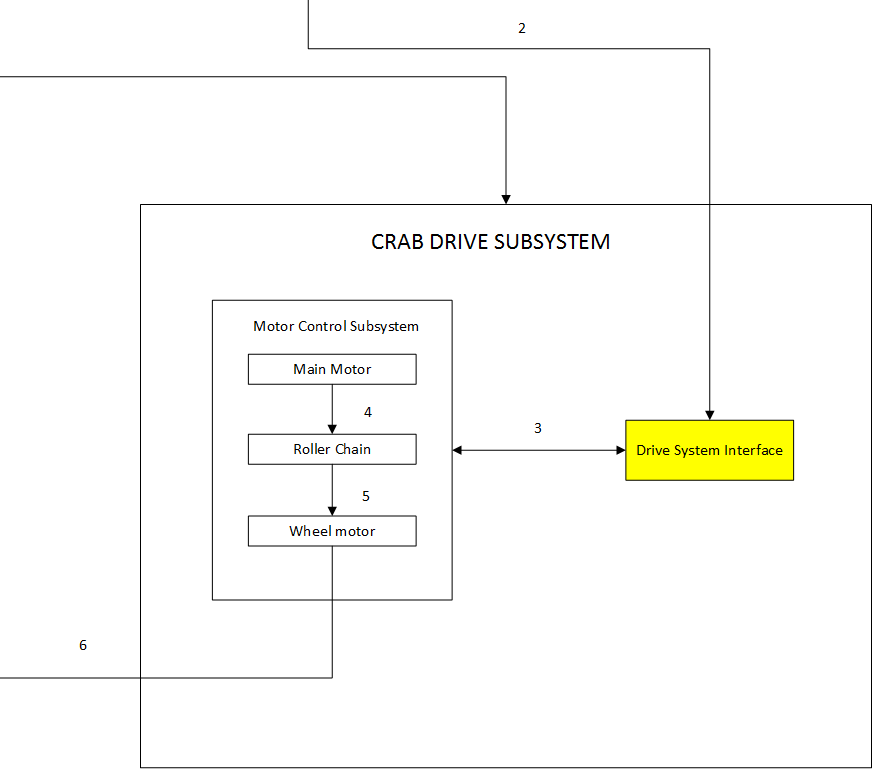
\includegraphics[width=0.60\textwidth]{images/drivesysteminterface}
 \caption{Drive system interface subsystem description diagram}
\end{figure}

\subsection{ASSUMPTIONS}
Assumptions made are as follows:
\begin{itemize}
\item The drive system interface will receive accurate navigation data from the camera interface.
\item The drive system will receive accurate feedback from the motor control subsystem.
\item The drive system interface will receive accurate feedback data from the main motor about wheel orientation
\end{itemize}

\subsubsection{RESPONSIBILITIES}
The responsibilites for drive system interface are as follows:
\begin{itemize}
\item Send navigation data to the motor control
\item Receive wheel feedback data
\end{itemize}

\subsubsection{DRIVE SYSTEM INTERFACE SUBSYSTEM INTERFACES}
\begin{table}[H]
\caption{Drive System Interface Subsystem Interface}
\begin{center}
\begin{tabular}{ | p{1cm} | p{6cm} | p{3cm} | p{3cm} |}
    \hline
    ID & Description & Inputs & Outputs \\ \hline
    \ 2 & Receive navigation data & \pbox{3cm}{Camera interface} & \pbox{3cm}{Motor Control}  \\ \hline
    \ 3 & Receive wheel data & \pbox{3cm}{Motor control} & \pbox{3cm}{Camera interface}  \\ \hline
\end{tabular}
\end{center}
\end{table}
\subsection{TEENSY MICRO-CONTROLLER}
A Teensy 3.2 micro-controller shall be used to control and coordinate the wheels via the motor-controllers.
\subsubsection{Subsystem Programming Languages}
The Teensy micro-controller shall be programmed in C++
\subsubsection{Subsystem Data Structures}
Data will be transmitted from a PC via USB to the Teensy.

\subsection{MOTOR CONTROLLERS}
The Smart Cart utilizes a Teensy Micro-controller in order to control the motorized wheels.
\subsubsection{Subsystem Programming Languages}
The motor controller shall be programmed in C++ and shall receive directional data from the micro-controller.

\newpage
\section{CART SUBSYSTEM}
The cart subsystem is largely the cart itself. it shall have pace for carrying user tools together with a charging area for user to put charging equipment, kill switch, manual mode switch and the wheels.

\subsection{MANUAL MODE SWITCH SUBSYSTEM}
The manual mode switch subsystem will be used to switch the cart to manual mode by disconnecting the power supply to the crab drive
\begin{figure}[h!]
	\centering
 	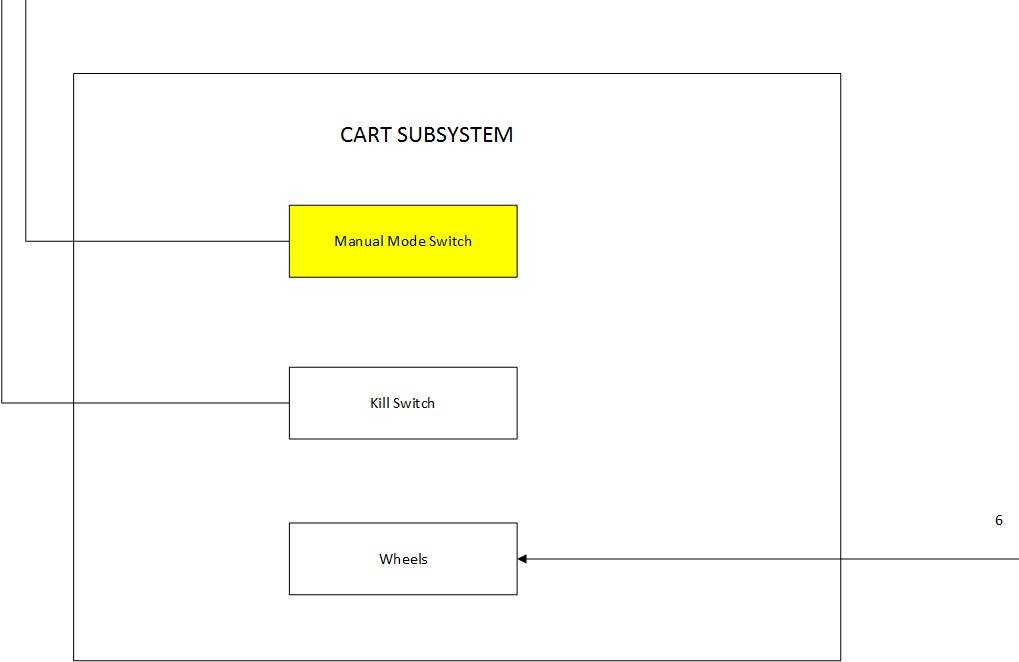
\includegraphics[width=0.60\textwidth]{images/manualmodeswitch}
 \caption{Manual Switch subsystem description diagram}
\end{figure}

\subsubsection{ASSUMPTIONS}
Assumptions made are as follows:
\begin{itemize}
\item The manual mode switch subsystem will ensure the safety of users and around the user
\item The manual mode switch subsystem will not power off Smart Cart, but simply disable autonomous motion  
\end{itemize} 

\subsubsection{RESPONSIBILITY}
The manual mode switch subsystem responsibilities are as follows:
\begin{itemize}
\item The switch will be used to disable the autonomous motion of the cart.
\item The switch will ensure safety of the users and the surrounding people
\end{itemize}

\subsubsection{Manual Mode Subsystem Interface}
\begin{table}[H]
\caption{Manual mode switch subsystem interface}
\begin{center}
\begin{tabular}{ | p{1cm} | p{6cm} | p{3cm} | p{3cm} |}
    \hline
    ID & Description & Inputs & Outputs \\ \hline
    \ N/A & Disable converter & \pbox{3cm}{N/A} & \pbox{3cm}{Voltage converter}  \\ \hline
\end{tabular}
\end{center}
\end{table}


\subsection{KILLSWITCH}
The killswitch subsystem will be used to ensure that the Smart Cart will be immediately turned off.
\begin{figure}[h!]
	\centering
 	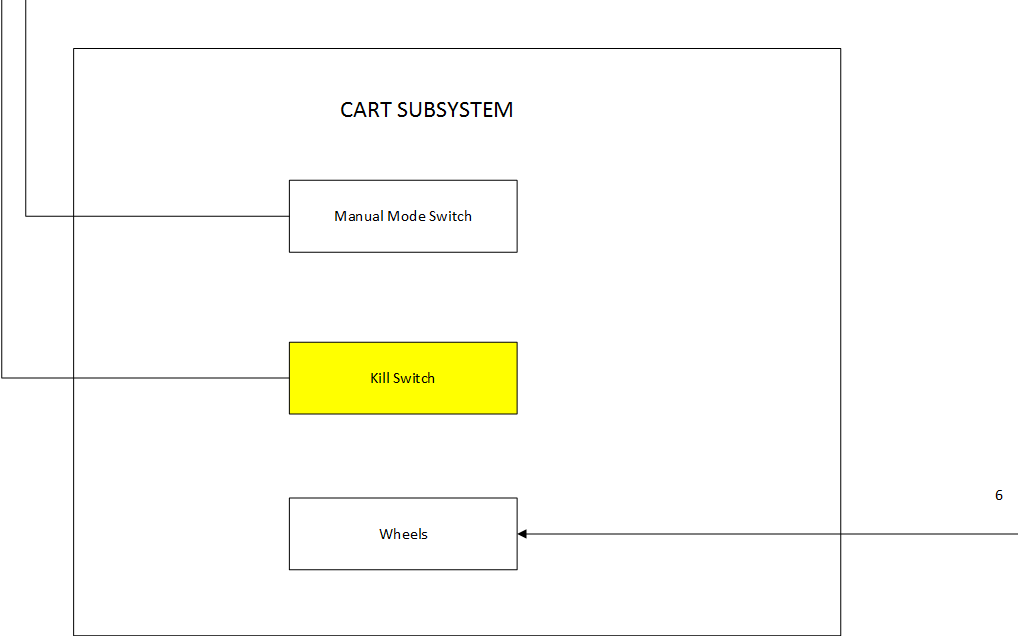
\includegraphics[width=0.60\textwidth]{images/killswitch}
 \caption{Kill Switch subsystem description diagram}
\end{figure}

\subsubsection{Assumptions}
Assumptions made are as follows:
\begin{itemize}
\item Power to Smart Cart components will be disabled
\item Power to external tools and equipment will be disabled
\end{itemize}

\subsubsection{RESPONSIBILITIES}
The killswitch subsystem responsibility are as follows:
\begin{itemize}
\item the switch will disable the battery from powering Smart Cart and its components
\end{itemize}

\subsubsection{Killswitch subsystem interface}
\begin{table}[H]
\caption{Sensors subsystem interface}
\begin{center}
\begin{tabular}{ | p{1cm} | p{6cm} | p{3cm} | p{3cm} |}
    \hline
    ID & Description & Inputs & Outputs \\ \hline
    \ N/A & Disable battery & \pbox{3cm}{N/A} & \pbox{3cm}{Deep cycle battery }  \\ \hline
\end{tabular}
\end{center}
\end{table}

\subsection{WHEEL SUBSYSTEM}
The wheels subsystem will be used to provide movement to the Smart Cart. The wheels will be controlled by the Crab Drive layer.
\begin{figure}[h!]
	\centering
 	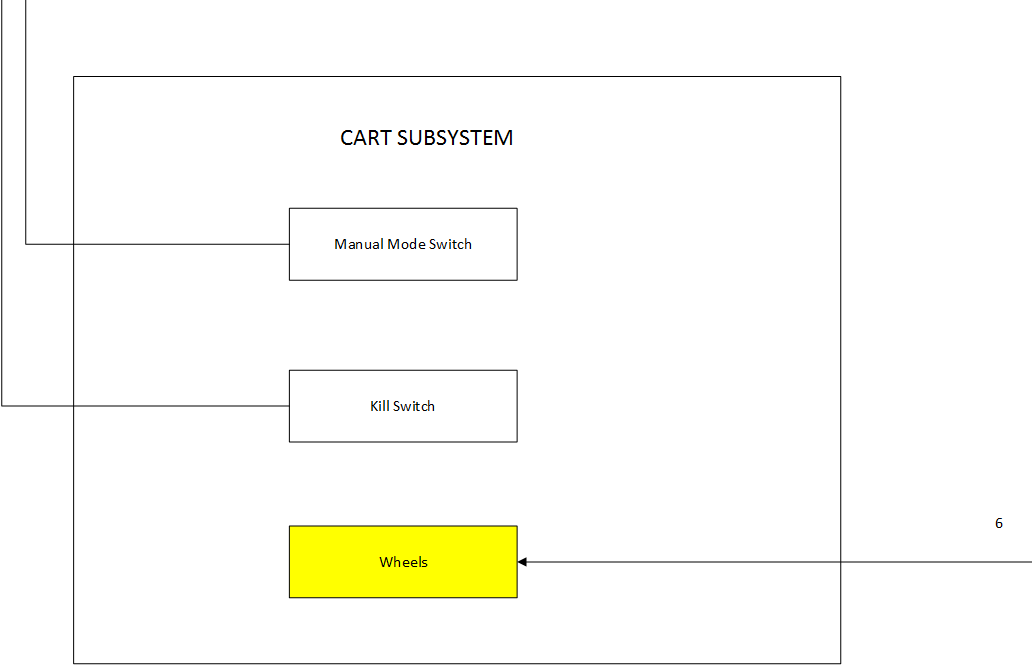
\includegraphics[width=0.60\textwidth]{images/wheels}
 \caption{Wheels subsystem description diagram}
\end{figure}

\subsubsection{ASSUMPTIONS}
Assumptions made are as follows:
\begin{itemize}
\item The wheels will be able to turn in the direction sort
\item The wheels will move harmoniously
\end{itemize}

\subsubsection{RESPONSIBILITIES}
The wheel subsystem responsibilities will be as follows
\begin{itemize}
\item Turn and move the cart from one point to anther
\item Take turns as directed by the wheel motors
\end{itemize}

\subsubsection{Wheel subsystem interfaces}
\begin{table}[H]
\caption{Sensors subsystem interface}
\begin{center}
\begin{tabular}{ | p{1cm} | p{6cm} | p{3cm} | p{3cm} |}
    \hline
    ID & Description & Inputs & Outputs \\ \hline
    \ 5 & Move Smart Cart & \pbox{3cm}{Wheel Motors} & \pbox{3cm}{N/A}  \\ \hline
\end{tabular}
\end{center}
\end{table}


\newpage
\section{Appendix A}
\subsection{CAD Design for Central Motor Sprocket}
\begin{figure}[h!]
	\centering
   	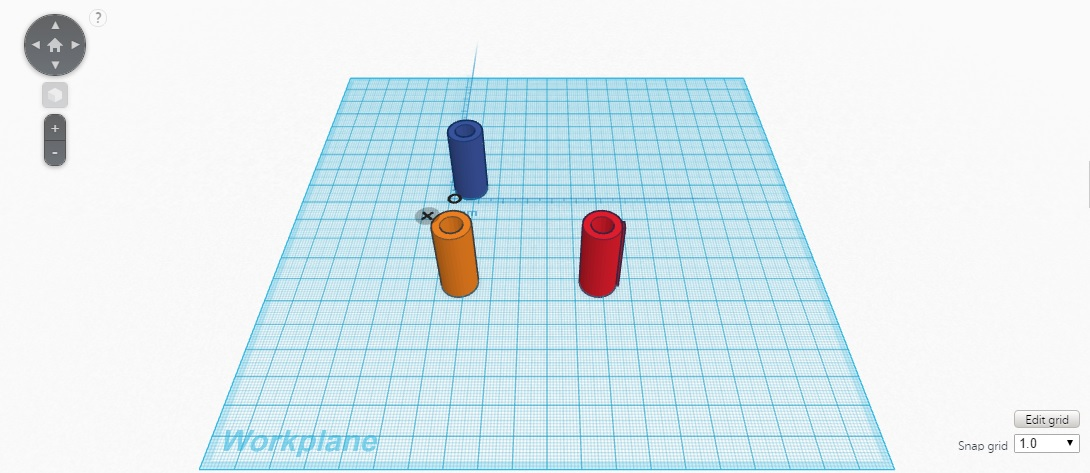
\includegraphics[width=0.60\textwidth]{images/CADimg}
\end{figure}

\subsection{Joystick Input Test Code}
\begin{verbatim}
//A0(15) = green, A1(16) = yellow, A2(17) = orange, A3(18) = red
#define downPin 15
#define upPin 16
#define rightPin 17
#define leftPin 18
int X = 0;
int Y = 0;
int PrevX = X;
int PrevY = Y;
 
void setup() {
  Serial.begin(9600);
  
  //Joystick setup
  pinMode(downPin, INPUT);
  digitalWrite(downPin, HIGH);
  pinMode(upPin, INPUT);
  digitalWrite(upPin, HIGH);
  pinMode(rightPin, INPUT);
  digitalWrite(rightPin, HIGH);
  pinMode(leftPin, INPUT);
  digitalWrite(leftPin, HIGH);
}

void loop() {
  joystick( &X, &Y );
  if (X != 0 && (X != PrevX || Y != PrevY)){
    result(X,Y);
  }
  else if (Y != 0 && (X != PrevX || Y != PrevY)) {
    result(X,Y);
  }
  delay(300);
}

// [-1, 0, 1] map to [left/down, none, right/top]
void joystick(int* X, int* Y){

  //HIGH = non-trigger
  if( !digitalRead( leftPin ) ){
    *X = -1;
  }else if( !digitalRead( rightPin ) ){
    *X = 1;
  }else{
    *X = 0;
  }

  if( !digitalRead( upPin ) ){
    *Y = 1;
  }else if( !digitalRead( downPin ) ){
    *Y = -1;
  }else{
    *Y = 0;
  }

}

void result(int X, int Y ) {
    if (X == 1){
      Serial.print("Right\t");
    }
    else if (X == -1) {
      Serial.print("Left\t");   
    }
    PrevX = X;
    if (Y == 1){
      Serial.print("Up\n");
    }
    else if (Y == -1) {
      Serial.print("Down\n");
    }
    else{
      Serial.print("\n");
    }          
    PrevY = Y;
}
\end{verbatim}

\subsection{Motor Driver Test Code}
\begin{verbatim}
/* LED Blink, Teensyduino Tutorial #1
   http://www.pjrc.com/teensy/tutorial.html
 
   This example code is in the public domain.
*/

// Teensy 2.0 has the LED on pin 11
// Teensy++ 2.0 has the LED on pin 6
// Teensy 3.x / Teensy LC have the LED on pin 13

//A0(15) = green, A1(16) = yellow, A2(17) = orange, A3(18) = red
const int LED_PIN = 13;
const int PWM_PIN = 14;
const int DIR_PIN = 10;
const int HB_PWM = 3;
const int HB_INA = 4;
const int HB_INB = 5;
const int DOWN_PIN = 15;
const int UP_PIN = 16;
const int RIGHT_PIN = 17;
const int LEFT_PIN = 18;
int X = 0;
int Y = 0;
int PrevX = X;
int PrevY = Y;

// the setup() method runs once, when the sketch starts
void setup() {
  // initialize the digital pin as an output.  
   Serial.begin(9600);
  
  pinMode(LED_PIN, OUTPUT);
  pinMode(PWM_PIN, OUTPUT);
  pinMode(DIR_PIN, OUTPUT);
  pinMode(HB_PWM, OUTPUT);
  pinMode(HB_INA, OUTPUT);
  pinMode(HB_INB, OUTPUT);
  pinMode(DOWN_PIN, INPUT);
  pinMode(UP_PIN, INPUT);
  pinMode(RIGHT_PIN, INPUT);
  pinMode(LEFT_PIN, INPUT);
  
  for(int i = 0; i < 25; i++)
  {
    digitalWrite(LED_PIN, HIGH);
    delay(50);
    digitalWrite(LED_PIN, LOW);
    delay(50);
  }
  
  digitalWrite(PWM_PIN, LOW);
  digitalWrite(DOWN_PIN, HIGH); 
  digitalWrite(UP_PIN, HIGH); 
  digitalWrite(RIGHT_PIN, HIGH); 
  digitalWrite(LEFT_PIN, HIGH); 
}

// the loop() methor runs over and over again,
// as long as the board has power
// pwm low = off
// 0 forward
void loop() {  
  joystick( &X, &Y );
  if (X != 0 && (X != PrevX || Y != PrevY)){
    result(X,Y);
  }
  else if (Y != 0 && (X != PrevX || Y != PrevY)) {
    result(X,Y);
  }
  delay(300);
}

void joystick(int* X, int* Y){
  //HIGH = non-trigger
  if( !digitalRead( LEFT_PIN ) ){
    *X = -1;
    turnLeft();
  }else if( !digitalRead( RIGHT_PIN ) ){
    *X = 1;
    turnRight();
  }else{
    *X = 0;
  }

  if( !digitalRead( UP_PIN ) ){
    *Y = 1;
    moveForward();
  }else if( !digitalRead( DOWN_PIN ) ){
    *Y = -1;
    moveBackward();
  }else{
    *Y = 0;
  }
}

void result(int X, int Y ) {
    if (X == 1){
      Serial.print("Right\t");
    }
    else if (X == -1) {
      Serial.print("Left\t");   
    }
    PrevX = X;
    if (Y == 1){
      Serial.print("Up\n");
    }
    else if (Y == -1) {
      Serial.print("Down\n");
    }
    else{
      Serial.print("\n");
    }          
    PrevY = Y;
}

void turnLeft() {
  digitalWrite(HB_PWM, HIGH);    
  digitalWrite(HB_INA, LOW); 
  digitalWrite(HB_INB, HIGH); 
  delay(1350); 
  digitalWrite(HB_PWM, LOW); 
}

void turnRight() {
  digitalWrite(HB_PWM, HIGH); 
  digitalWrite(HB_INB, LOW); 
  digitalWrite(HB_INA, HIGH);
  delay(1350); 
  digitalWrite(HB_PWM, LOW);
}

void moveForward() {
  digitalWrite(PWM_PIN, HIGH);
  digitalWrite(DIR_PIN, HIGH);
  delay(1000);
  digitalWrite(PWM_PIN, LOW);
}

void moveBackward() {
  digitalWrite(PWM_PIN, HIGH);
  digitalWrite(DIR_PIN, LOW);
  delay(1000);
  digitalWrite(PWM_PIN, LOW);
}
\end{verbatim}

\subsection{Final Demo Code}
\begin{verbatim}
const int LED_PIN = 13;
const int PWM_PIN = 10;
const int DIR_PIN = 14;
const int HB_PWM = 3;
const int HB_INA = 4;
const int HB_INB = 5;
const int DOWN_PIN = 15;
const int UP_PIN = 16;
const int RIGHT_PIN = 17;
const int LEFT_PIN = 18;

int X = 0;
int Y = 0;
int PrevX = X;
int PrevY = Y;

void setup() {
  Serial.begin(9600);
  
  pinMode(LED_PIN, OUTPUT);
  pinMode(PWM_PIN, OUTPUT);
  pinMode(DIR_PIN, OUTPUT);
  pinMode(HB_PWM, OUTPUT);
  pinMode(HB_INA, OUTPUT);
  pinMode(HB_INB, OUTPUT);
  pinMode(DOWN_PIN, INPUT);
  pinMode(UP_PIN, INPUT);
  pinMode(RIGHT_PIN, INPUT);
  pinMode(LEFT_PIN, INPUT);
  
  for(int i = 0; i < 25; i++)
  {
    digitalWrite(LED_PIN, HIGH);
    delay(50);
    digitalWrite(LED_PIN, LOW);
    delay(50);
  }

  analogWrite(HB_PWM, LOW);
  digitalWrite(PWM_PIN, LOW);
  digitalWrite(DOWN_PIN, HIGH); 
  digitalWrite(UP_PIN, HIGH); 
  digitalWrite(RIGHT_PIN, HIGH); 
  digitalWrite(LEFT_PIN, HIGH); 
}

void loop() {
  joystick( &X, &Y );
  if (X == 0  && Y == 0){
    stopMoving();
  }
  if (X != 0 && Y != 0){    
    result(X,Y);
  }
 /* stopMoving();
  delay(3000);
  moveForward();
  delay(2000);
  stopMoving();
  delay(3000);
  moveBackward();
  delay(2000);*/
}

void joystick(int* X, int* Y){
  if( !digitalRead( UP_PIN ) ){
      *Y = 1;
      moveForward();
  } else if( !digitalRead( DOWN_PIN ) ){
      *Y = -1;
      moveBackward();
  } else{
      *Y = 0;
  }

  if( !digitalRead( LEFT_PIN ) ){
    *X = -1;
    if (*Y == -1){
      turnLeft();
    } else {
        turnRight();
    }
  } else if( !digitalRead( RIGHT_PIN ) ){
    *X = 1;
    if (*Y == -1){
      turnRight();
    }
    else {
      turnLeft();
    }
  } else{
    *X = 0;
  }
}

void result(int X, int Y ) {
    Serial.print( "X = ");
    Serial.print(X);
    Serial.print(" Y = ");
    Serial.print(Y);
    Serial.print('\n');
    
    PrevX = X;
    PrevY = Y;
}

void turnLeft(){
  digitalWrite(HB_PWM, HIGH);
  digitalWrite(HB_INA, LOW);
  digitalWrite(HB_INB, HIGH);
}

void turnRight(){
  digitalWrite(HB_PWM, HIGH);
  digitalWrite(HB_INB, LOW);
  digitalWrite(HB_INA, HIGH);
}

void moveForward(){
  analogWrite(PWM_PIN, 80);
  digitalWrite(DIR_PIN, HIGH);
}

void moveBackward(){
  analogWrite(PWM_PIN, 80);
  digitalWrite(DIR_PIN, LOW);
}

void stopMoving(){
 analogWrite(PWM_PIN, LOW);
 digitalWrite(HB_PWM, LOW); 
 digitalWrite(HB_INA, LOW); 
 digitalWrite(HB_INB, LOW); 
}
\end{verbatim}

\newpage

%%% References
\bibliographystyle{plain}
\bibliographystyle{reference/IEEEtran_custom}
\bibliography{reference/refs}{}

\end{document}